\section{Exercise 7.11: The DFT of a cosine} 

% Code listing configuration for MATLAB
\lstset{
    language=Matlab,
    basicstyle=\ttfamily\small,
    keywordstyle=\color{blue},
    stringstyle=\color{purple},
    commentstyle=\color{green!60!black},
    numbers=left,
    numberstyle=\tiny\color{gray},
    breaklines=true,
    frame=single,
    captionpos=b
}

\subsection{MATLAB Implementation}

\lstinputlisting[caption={MATLAB script \texttt{dft\_cosine.m}}, label={lst:dft_cosine}]{Code/dft_cosine.m}


\subsection{Results}

\begin{figure}[H]
    \centering
    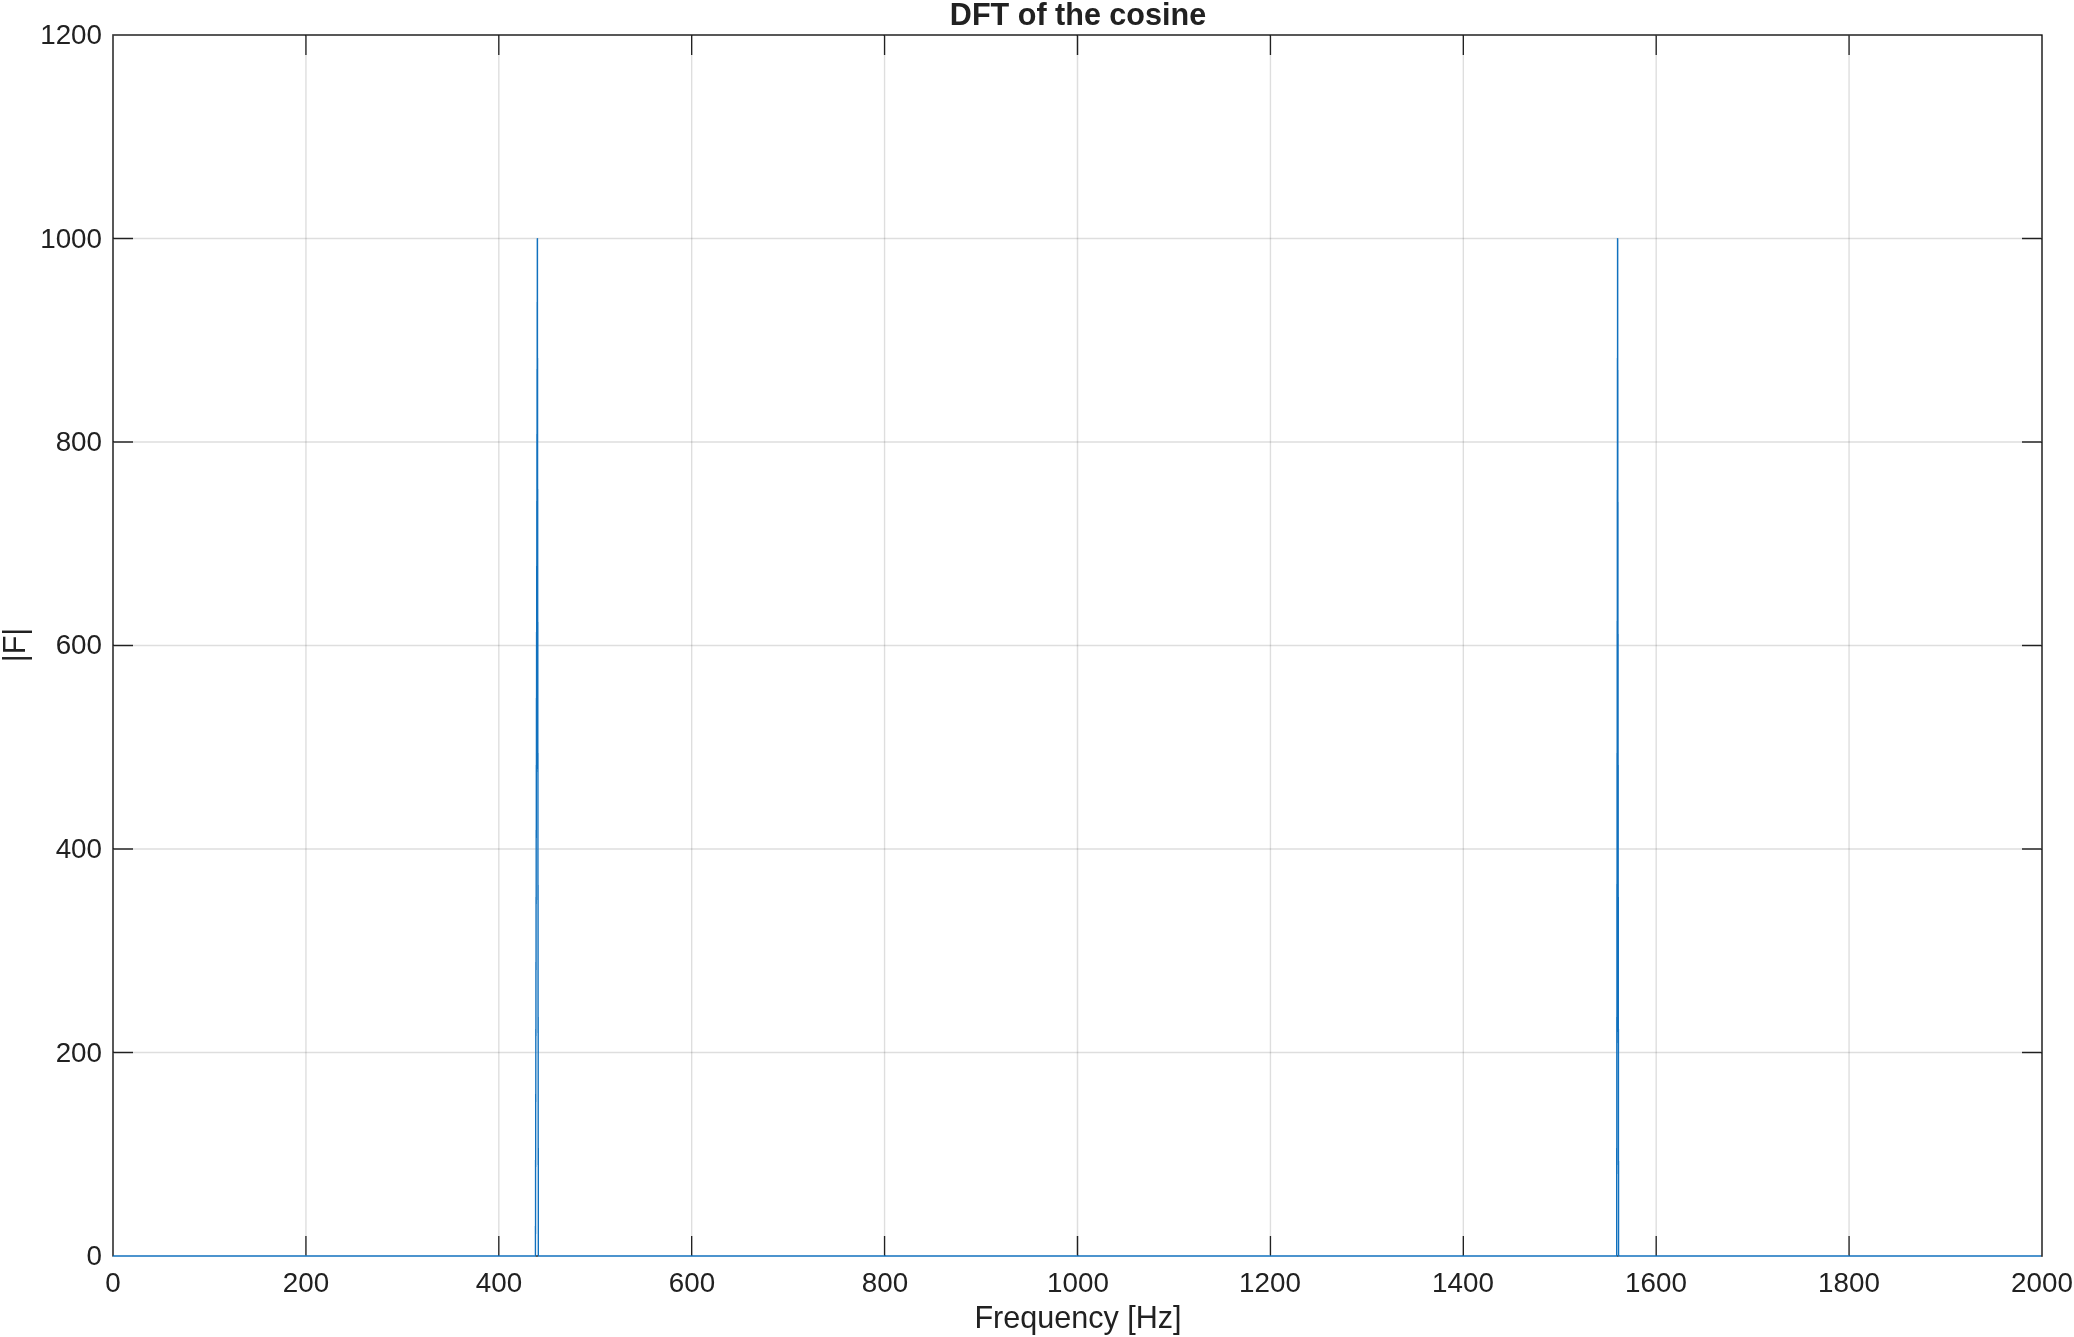
\includegraphics[width=1\linewidth]{Figures//7.11 Figures/Raw DFT of sampled cosine.png}
    \caption{Raw DFT of sampled cosine}
    \label{fig:placeholder}
\end{figure}

\begin{figure}[H]
    \centering
    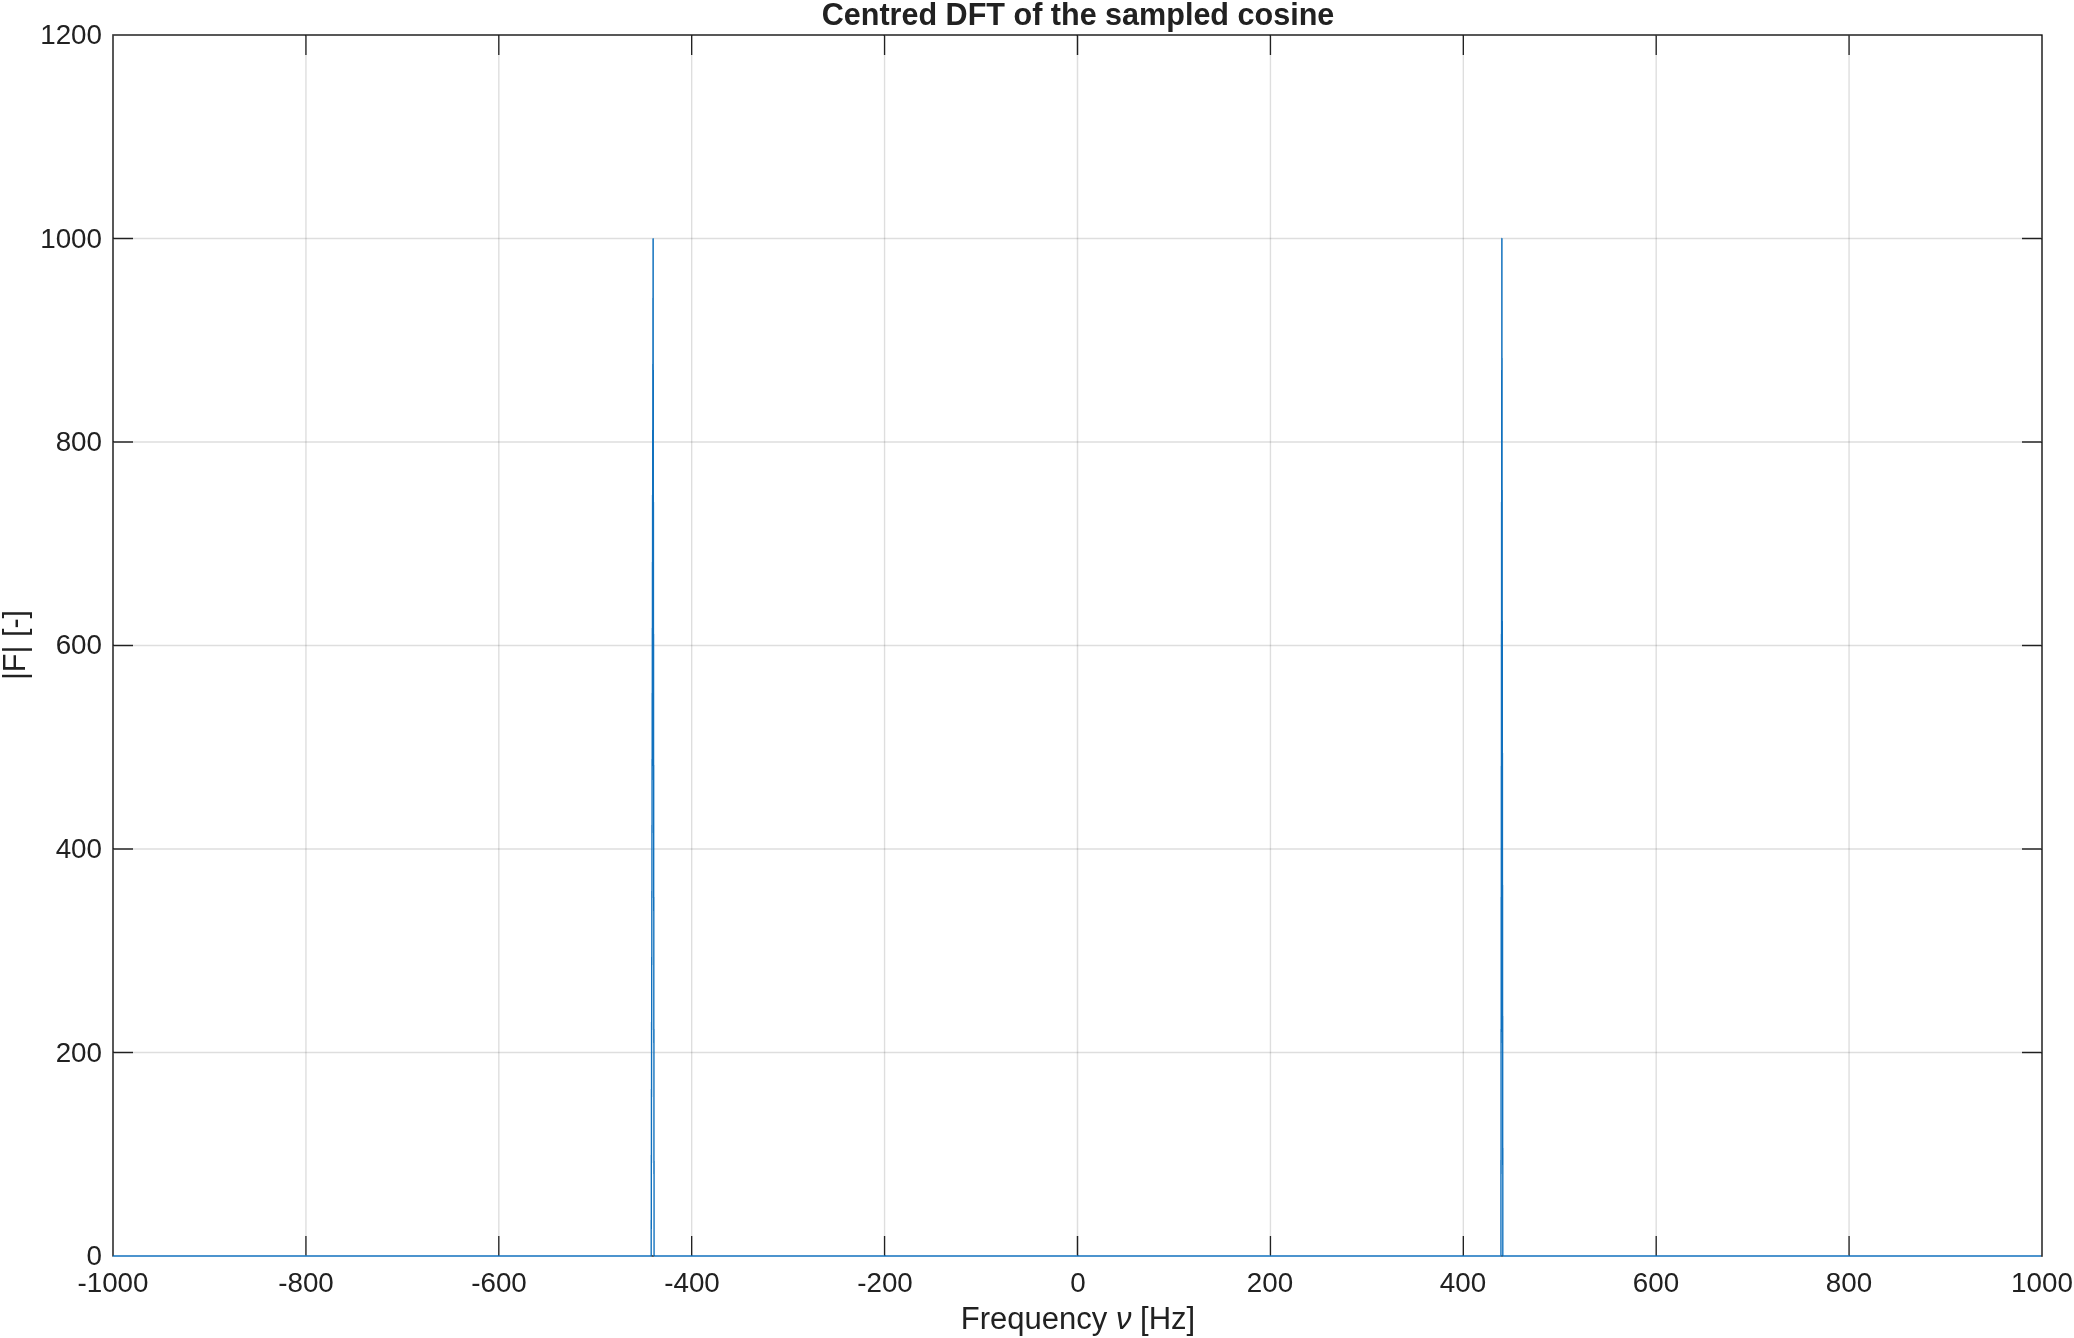
\includegraphics[width=1\linewidth]{Figures//7.11 Figures/Centered DFT of the sampled cosine.png}
    \caption{Centered DFT of the sampled cosine}
    \label{fig:placeholder}
\end{figure}

\begin{figure}[H]
    \centering
    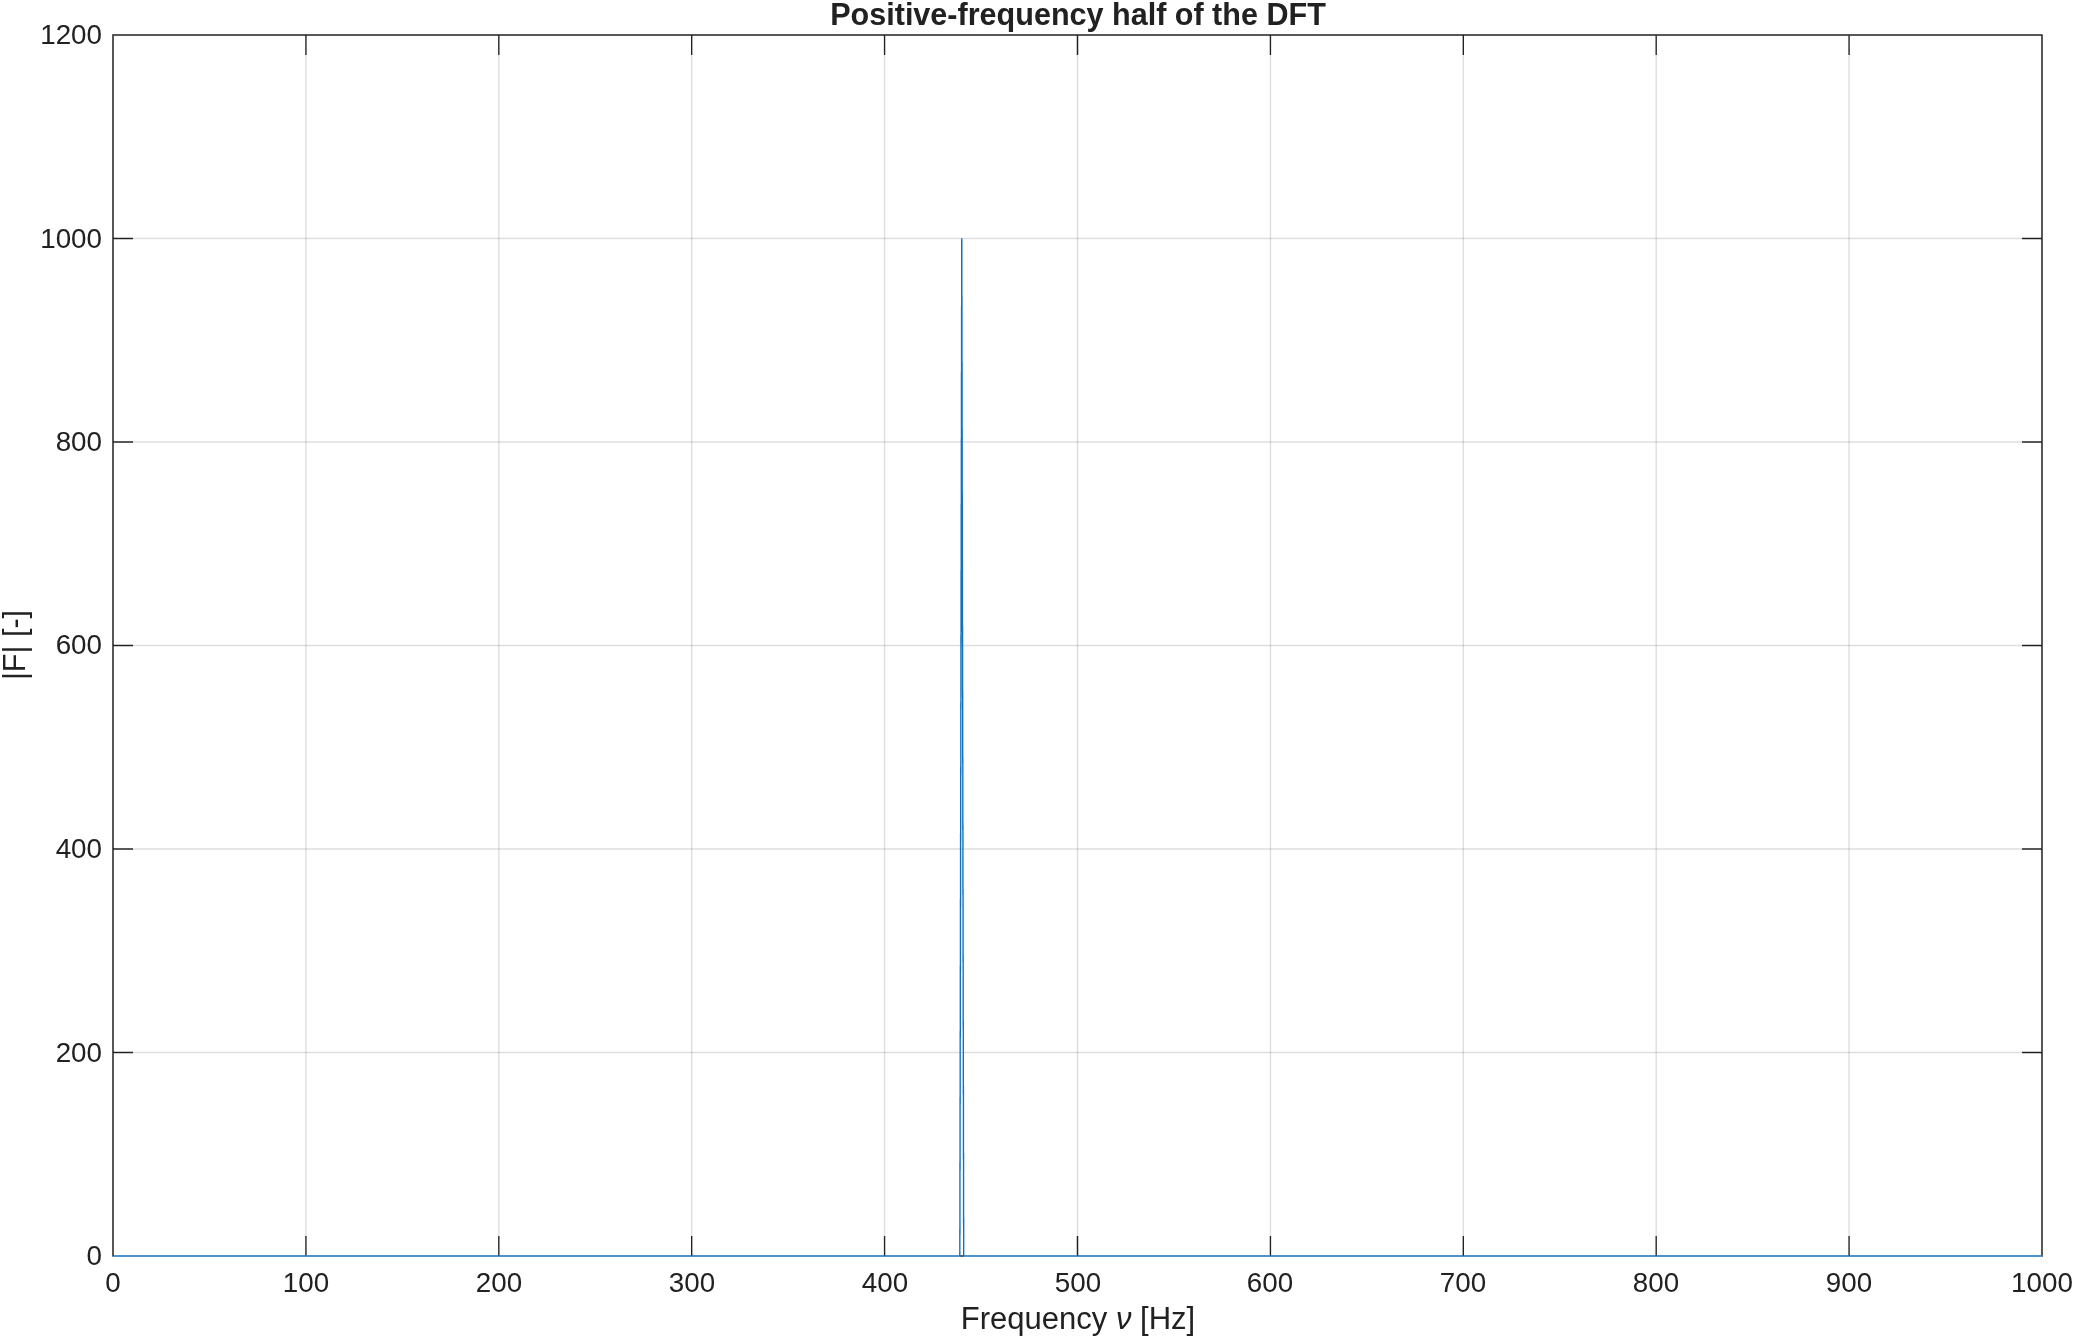
\includegraphics[width=1\linewidth]{Figures//7.11 Figures/Positive frequency half of the DFT.png}
    \caption{Positive frequency half of the DFT}
    \label{fig:placeholder}
\end{figure}


\subsection{Results Analysis}

The first value of the DFT array is $\nu$=0 Hz, with a frequency resolution of $\Delta\nu = \frac{1}{\Delta t}$, so a signal duration of 1s leads to a frequency resolution of $\Delta\nu = 1$ Hz.
\\
\\
The $N_s$ samples of the DFT array are $\nu_k = k\Delta \nu = \frac{k\nu_s}{N_s}$, where k runs from 0 to $N_s-1$. For our defined $N_s = 2000$, these values run from 0 to 1999.
\\
\\
\textbf{Question 3}
\\
For
\[
f(t)=\cos(\omega_0 t),
\]
the continuous Fourier transform is
\[
F(\omega)=\pi\left[\delta(\omega-\omega_0)+\delta(\omega+\omega_0)\right].
\]

So, peaks are expected at $\nu = \pm440$ Hz.

The centred DFT supports this, as peaks are seen at $\nu = -440$Hz and $\nu = +440$ Hz

In the unshifted DFT, the frequency component at -440 Hz appears at 
appears at
\[
\nu_s-440
=
2000-440
=
1560\,\mathrm{Hz}.
\]

Therefore, the unshifted DFT has peaks at 440 Hz and 1560 Hz.
\\
\\
\textbf{Question 4}
\\
For a real-valued function, the negative and positive parts of the DFT contain the same magnitude information. This is known as conjugate symmetry.
\[
F[N-k]=F^*[k],
\]
so
\[
|F[N-k]|=|F[k]|.
\]
Therefore, for a real signal, only plotting the lower-half or positive frequency  half of the spectrum is sufficient, as each part is essentially a mirror of eachother.
\\
\\
\textbf{Question 5}
\\
The sampling frequency to $\nu_s = 2000$ Hz leads to a Nyquist frequency of $\nu_N = \nu_s/2 = 1000$ Hz. With a $v_0$ = 1800 Hz, 1800>1000. This will lead to aliasing, due to the periodic behaviour of the frequency spectrum. Therefore, shifting will lead to peaks appearing at 2000-1800=$ 200$ Hz. This means the sampled 1800 Hz cosine is indistinguishable from a 200Hz cosine, at the given sampling frequency.
\\
\\
\textbf{Question 6}
\\
The relation between the signal duration and frequency resolution of the DFT is defined by
\[
\Delta t = 0.1\,\mathrm{s},
\]
For $\Delta t$=0.1s a frequency resolution of $\Delta\nu = 10$Hz is obtained. This means the spacing between frequency bins is wider, which results in a lower frequency resolution.
For $\Delta t$=10s, the frequency resolution becomes $\Delta\nu=0.1$ Hz. This leads to less spacing between frequency bins, which results in a higher frequency resolution.
\\
\\

Changing frequency resolution does not shift the peak, as it remains at approximately $v_0 = 440$Hz. However, increasing the signal duration results in a more finely sampled frequency spectrum, and the magnitude of the DFT peak also changes because the number of samples changes. Since MATLAB's \texttt{fft} is not normalised, the magnitude of each cosine peak is approximately

\[
\frac{N_s}{2}.
\]

Therefore, increasing $\Delta t$ also increases the magnitude of the peak because more samples are included in the DFT.
